\documentclass{article}

\usepackage{graphicx}
\usepackage{tikz}
\usepackage{tikzsymbols}
\usetikzlibrary{calc,patterns,shapes.geometric}
\pagestyle{empty}
\usepackage[margin=0pt]{geometry}
\geometry{papersize={14in,12in}}

\def\centerarc[#1](#2)(#3:#4:#5){\draw[#1] ($(#2)+({#5*cos(#3)},{#5*sin(#3)})$) arc (#3:#4:#5);}

\begin{document}
	\begin{figure}
		\centering
		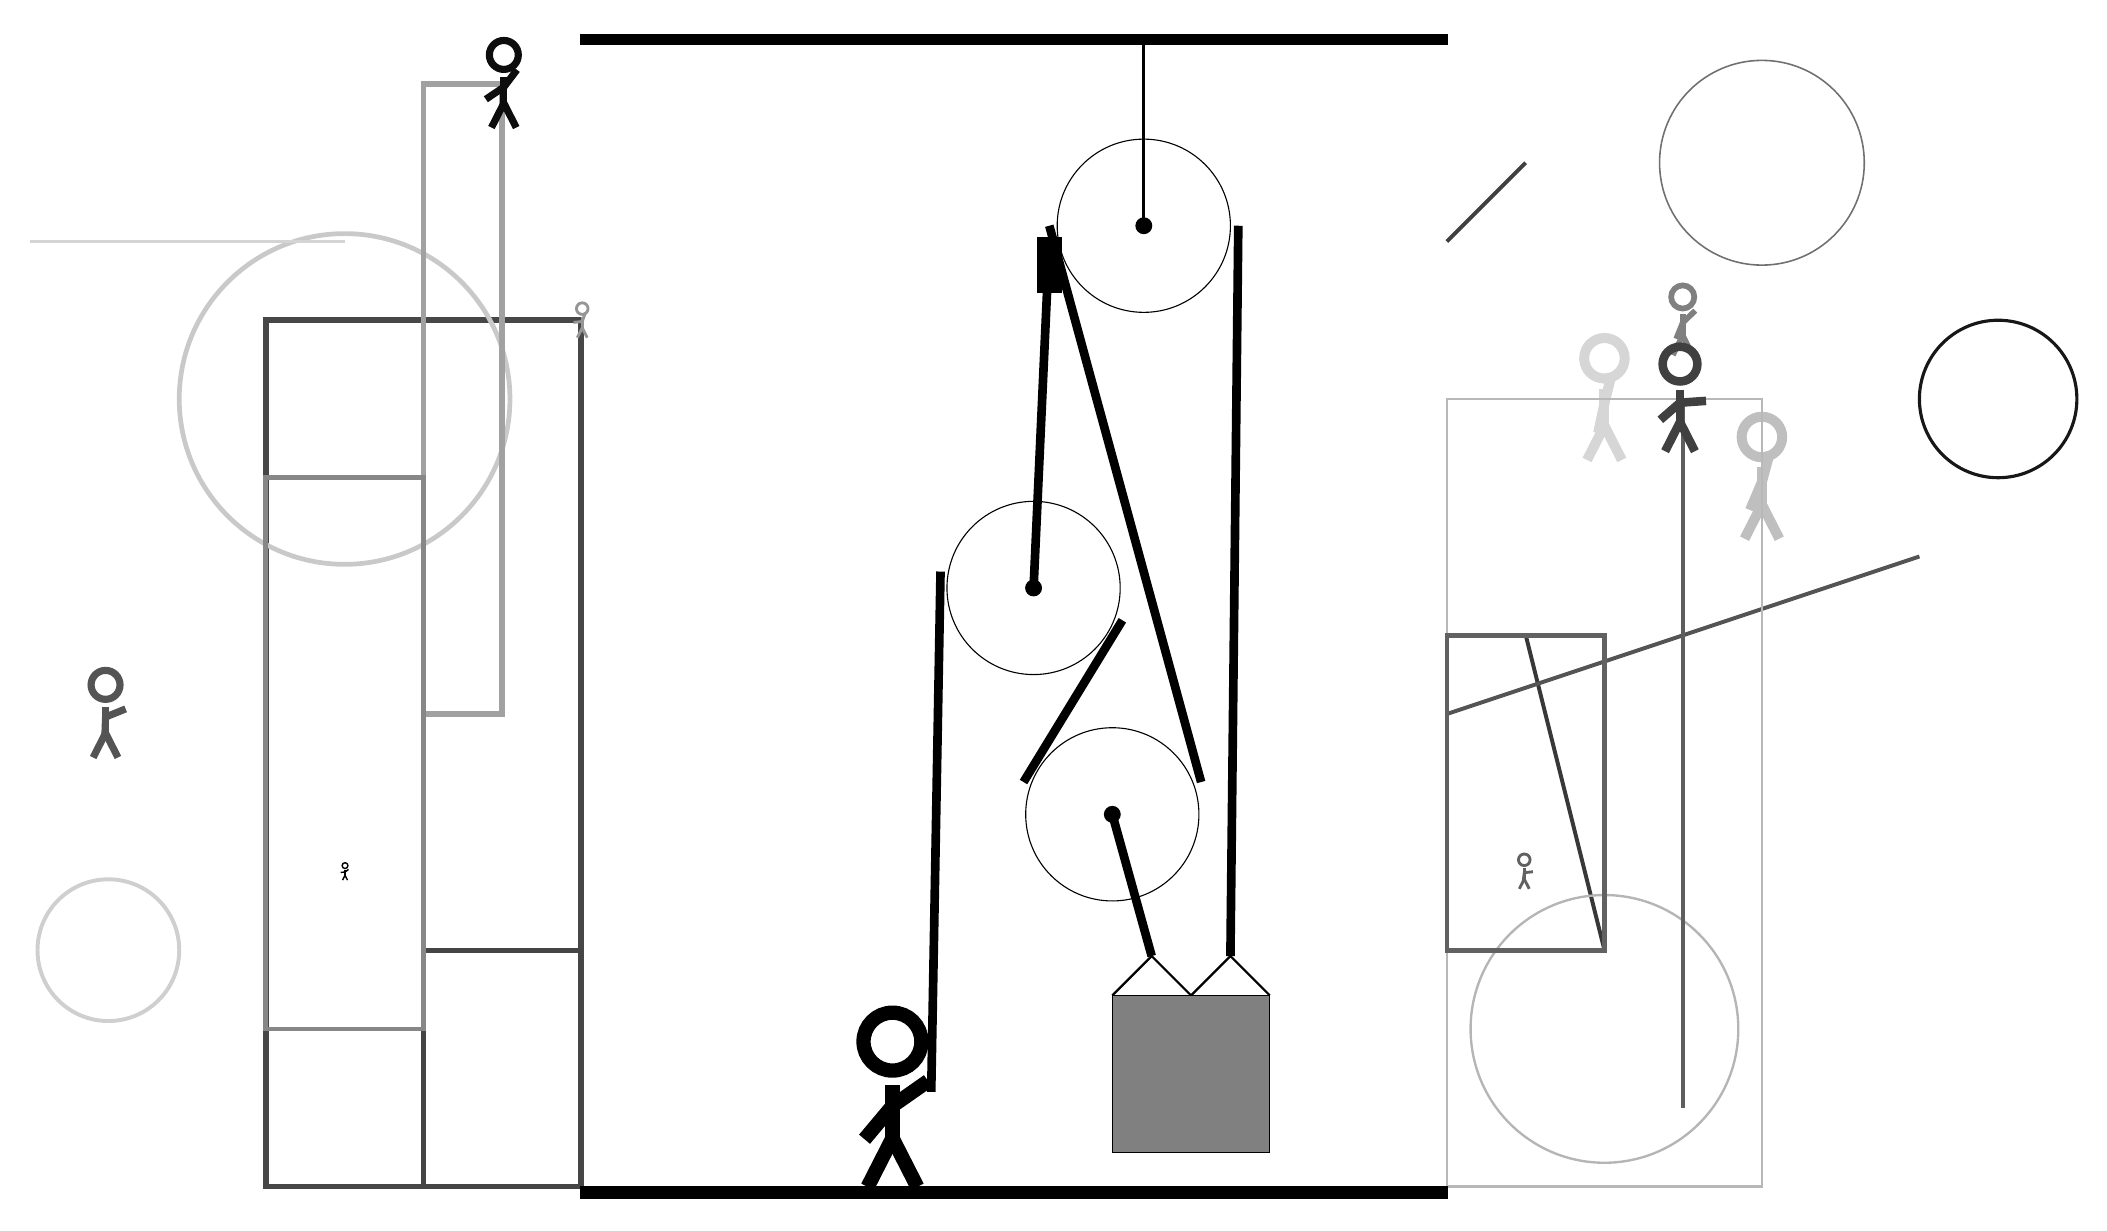
\begin{tikzpicture}
			%%%%% START %%%%%
			
			\draw[fill=black] (-6, 11.5) rectangle (5, 11.625);
			
			\draw (-0.25, 4.6) circle (1.1);
			\draw[fill=black] (-0.25, 4.6) circle (0.1);
			
			\draw (0.75, 1.725) circle (1.1);
			\draw[fill=black] (0.75, 1.725) circle (0.1);
			
			\draw (1.15, 9.2) circle (1.1);
			\draw[fill=black] (1.15, 9.2) circle (0.1);
			\draw[very thick] (1.15, 9.2) -- (1.15, 11.5);
			
			\draw[thick]  (0.75, -0.575) -- (1.25, -0.075) -- (1.75, -0.575) -- (2.25, -0.075) -- (2.75, -0.575);
			\draw[fill=black!50] (0.75, -0.575) rectangle (2.75, -2.575);
			
			\draw[line width=0.7mm, color=black!72] (-6, -3) rectangle (-10, 8);
			
			\draw[line width=0.5mm, color=black!78](7, 0) -- (6, 4);
			\draw [line width=0.3mm, color=black!29](7, -1) circle (1.7);
			\node[line width=0.4mm, color=black!50] at (8, 8) {\Strichmaxerl[4][68][44]};
			
			\draw [line width=0.6mm, color=black!21](-9, 7) circle (2.1);
			\node[line width=0.5mm, color=black!16] at (7, 7) {\Strichmaxerl[7][78][76]};
			\node[line width=0.4mm, color=black!25] at (9, 6) {\Strichmaxerl[7][67][75]};
			\draw[line width=0.5mm, color=black!67](5, 3) -- (11, 5);
			\draw[line width=0.5mm, color=black!63](8, -2) -- (8, 7);
			\draw[line width=0.7mm, color=black!37] (-8, 11) rectangle (-7, 3);
			\node[line width=0.2mm, color=black!95] at (-7, 11) {\Strichmaxerl[5][34][53]};
			
			\draw [line width=0.2mm, color=black!56](9, 10) circle (1.3);
			\draw[line width=0.3mm, color=black!28] (5, 7) rectangle (9, -3);
			
			\draw[line width=0.6mm, color=black!73] (-6, -3) rectangle (-8, 0);
			\draw[line width=0.6mm, color=black!47] (-8, 6) rectangle (-10, -1);
			\node[line width=0.3mm, color=black!62] at (6, 1) {\Strichmaxerl[2][83][6]};
			\node[line width=0.3mm, color=black!41] at (-6, 8) {\Strichmaxerl[2][6][70]};
			
			\draw[line width=0.5mm, color=black!75](6, 10) -- (5, 9);
			\node[line width=0.3mm, color=black!67] at (-12, 3) {\Strichmaxerl[5][88][22]};
			
			\node[line width=0.3mm, color=black!100] at (-9, 1) {\Strichmaxerl[1][5][37]};
			\draw [line width=0.4mm, color=black!91](12, 7) circle (1.0);
			\draw[line width=0.5mm, color=black!17](-9, 9) -- (-13, 9);
			\draw [line width=0.5mm, color=black!19](-12, 0) circle (0.9);
			\draw[line width=0.6mm, color=black!62] (5, 4) rectangle (7, 0);
			\node[line width=0.3mm, color=black!75] at (8, 7) {\Strichmaxerl[6][41][4]};
			
			
			\draw[line width=1.1mm] (-0.25, 4.6) -- (-0.05, 9.0);
			\draw[line width=1.1mm, fill=black](-0.15, 8.4) rectangle (0.05, 9.0);
			\draw[line width=1.1mm] (-1.55, -1.8) -- (-1.4318, 4.8083);
			\centerarc[line width=1.1mm](-0.25, 4.6)(-20:170:1.2000000000000002);
			\draw[line width=1.1mm] (0.8776, 4.1896) -- (-0.3776, 2.1354);
			\centerarc[line width=1.1mm](0.75, 1.725)(160:380:1.2000000000000002);
			\draw[line width=1.1mm] (1.8776, 2.1354) -- (-0.05, 9.2);
			\draw[line width=1.1mm](0.75, 1.725) -- (1.25, -0.075);
			\centerarc[line width=1.1mm](1.15, 9.2)(0:180:1.2000000000000002);
			\draw[line width=1.1mm] (2.35, 9.2) -- (2.25, -0.075);
			
			\node at (-2, -1.9) {\Strichmaxerl[10][50][35]};
			
			\draw[fill=black] (-6, -3) rectangle (5, -3.15);
			
			%%%%% END %%%%%
		\end{tikzpicture}
	\end{figure}	
\end{document}